\section{Approach}
Plenty of literature exists on modeling both surface rail networks, which typically cover longer distances, and subway or light-rail systems, which typically operate with a higher train frequency. Whereas simulations of surface rail networks might focus on maintaining arrival and departure schedules, subway and metro systems are more interested in keeping the trains moving and avoiding deadlock.  Deadlock is a state where no train can advance.  For example, consider a scenario where a train is broken down for an extended period of time.  As time advances, trains continue to arrive behind the disabled train, but are unable to pass.  Eventually all trains are stuck behind the disabled train.  Careful placement and management of track switches can be used to allow trains to overtake and pass a disabled train. These management schemes require modeling and simulation to evalueate their effectiveness.  According to Ref.~\citen{ttcservice}, Toronto subway trains run every two to seven minutes. Even small delays of just a couple minutes can result in relatively significant delays.

The approach considered here consists of five atomic components coupled together: stations, track sections, trains, passengers and a scheduler. Stations and track sections are modeled similarly, with the exception that passengers can be unloaded and loaded at stations. Two tracks, one for each direction, join stations together. Each train carries up to a specified maximum number of passengers. The time to load and unload passengers is linearly dependent on the number of passengers involved in the operations. Passengers originate and terminate at stations.  Trains may also suffer from failures, which cause delays in service.  The role of the scheduler is to control the motion of the trains and ensure no collisions or deadlocks occur.  The models for these components are described in more detail in the following sections.

\subsection{Rail System Models}
A natural data structure choice for representing a rail system is a directed graph.  In the most basic implementation, each station would be a vertex and the edges would each represent a directional track from one station to the next. Figure~\ref{fig:directedgraph} shows a directed graph model of the Sheppard Line in the Toronto subway system.
\begin{figure}[htb]
	\centering
	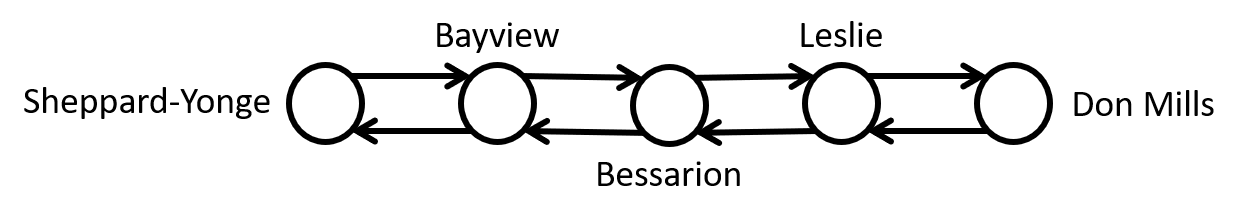
\includegraphics[width=6.5in]{directedgraph.png}
	\caption{Directed Graph Model of Sheppard Subway Line}
	\label{fig:directedgraph}
\end{figure}
What the directed graph representation lacks for this application is any notion of an integrated train model. A separate train model could be made to use the directed graph simply to know where to go next, but it would require much extra logic to determine \textit{if} it could go do the next station.  Where this decision is made is also not obvious when using the directed graph.

Similar to directed graphs and used in discrete event modeling of concurrent systems is a structure called a Petri net.~\cite{Petri62}  Synonymous to the vertices in a directed graph, Petri nets contain \textit{places}.  Whereas directed graphs use edges to connect those vertices, Petri nets use \textit{arcs}. However, Petri nets do not simply connect one \textit{place} to another.  \textit{Arcs} actually connect \textit{places} to \textit{transitions}. Each \textit{transition} has an input and an output arc joining it to \textit{places}.  Each \textit{place} optionally can contain a finite number of \textit{tokens}.  \textit{Tokens} for this application represent the trains.  More formally, they are objects that represent processes in a given state, where the states are represented by the \textit{places}.~\cite{Kristoffersen2003}  Figure~\ref{fig:petrinet} shows a Petri net model of the Sheppard subway line. The rectangles at the midpoint of the arcs represent the transitions and the black dots inside the represent the tokens.
\begin{figure}[htb]
	\centering
	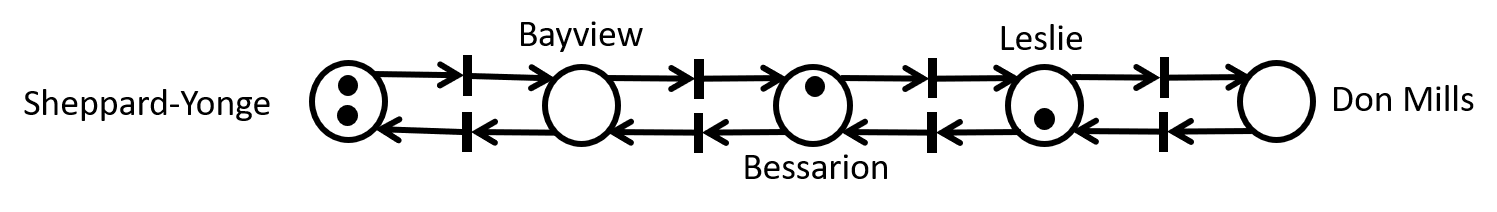
\includegraphics[width=6.5in]{petrinet.png}
	\caption{Petri Net Model of Sheppard Subway Line}
	\label{fig:directedgraph}
\end{figure}

\subsection{Track Section Model}

The track section model is needed to control access to track sections. A train
is permitted to enter a section if their is remaining capacity in the section.
When a train leaves a section the section's remaining capacity is increased by
one. The track section model can be represented by the model below.

\newcommand{\InEnterReq}[0]{(\text{``Enter Request''}, ())}
\newcommand{\InExitReq}[0]{(\text{``Exit Request''}, ())}

\newcommand{\OutEnterRes}[1]{(\text{``Enter Response''}, #1)}

\begin{align*}
    A &= \text{Number of trains allowed on section} \\
    X &= \{\InEnterReq, \\
        & \InExitReq
    \} \\
    Y &= \{\OutEnterRes{\{\text{May enter}, \text{May not enter}\}}\} \\
    S &= \{ a | a \in \mathbb{N}_0, a \leq A \} \\
    ta(S) &= \infty \\
    \delta_{ext}(a, e, \InEnterReq) &= 
        \begin{cases}
            a - 1 & \text{if\;} a > 0 \\
            a & \text{otherwise} \\
        \end{cases} \\
    \delta_{ext}(a, e, \InExitReq) &= 
        \begin{cases}
            a + 1 & \text{if\;} a < A \\
            a & \text{otherwise} \\
        \end{cases} \\
    \lambda(a) &= 
        \begin{cases}
            \text{May enter} & \text{if\;} a > 0 \\
            \text{May not enter} & \text{otherwise} \\
        \end{cases}
\end{align*}

\subsection{Train Model}

Trains travel station to station to unload and load passengers. Sometimes they
break down. They also recieve instructions or signals to break down or move
forward. This behaviour is represented by the model below. Any missing
transitions are assumed to return the input state. 

The model makes some simplifying assumptions. It assumes that each track section
includes stations and the track up to the next station. This assumption could be
relaxed by having the train keep track of whether or not the train is at a
station. A 50\% disembark rate is also assumed for unloading at each station. A
more detailed model would include each passengers destination station so that
forced breakdowns event would force passengers to exit and those that did not
reach their desired destination would board the next train (this model assumes
disembarkers never reboard). It also assumes that breakdown repair times and in
need of repair times is constant.

\newcommand{\InBreakDown}[0]{(\text{``Breakdown''}, ())}
\newcommand{\InCapReq}[0]{(\text{``Capacity Request''}, ())}
\newcommand{\InMoveRes}[1]{(\text{``Move Response''}, #1)}
\newcommand{\InLoadPassengers}[1]{(\text{``Load Passengers''}, #1)}

\newcommand{\OutRemainingCapacity}[1]{(\text{``Remaining Capacity''}, #1)}
\newcommand{\OutUnloadPassengers}[1]{(\text{``Unload Passengers''}, #1)}
\newcommand{\OutMoveReq}[0]{(\text{``Move Request''}, ())}
\newcommand{\phase}[0]{\text{phase}}

\newcommand{\Mod}[2]{\mathrm{mod} (#1, #2)}

\begin{align*}
    N &= \# \text{\;of train stations} \\
    C &= \text{Passenger capacity of train} \\
    X &= \{
      \InBreakDown, \\
      &  \InCapReq, \\
      &  \InLoadPassengers{\{ p | p \in \mathbb{N}_0, p \leq C \}} \\
      &  \InMoveRes{\{ \text{Accepted}, \text{Rejected} \}}
    \} \\
    Y &= \{
      \OutRemainingCapacity{\{ c | c \in \mathbb{N}_0 \}}, \\
      &  \OutUnloadPassengers{\{ u | u \in \mathbb{N}_0 \}}, \\
      &  \OutMoveReq
    \} \\
    S_{action} &= \{
      \text{moving}, \text{needs repairs}, \text{in repair}, \\
      &  \text{loading}, \text{unloading}, \text{waiting} 
    \} \\
    S_{\text{position}} &= \{ i | i \in \mathbb{N}_0, i \leq N
    \} \\
    S_{passengers} &= \{ p | p \in \mathbb{N}_0, p \leq C \} \\
    S &= S_{action} \times S_{position} \times S_{passengers} \times \sigma \\
    ta(a, i, p, \sigma) &= \sigma \\
    \delta_{ext}((\text{moving}, i, p, \sigma), e, \InBreakDown) &= 
        (\text{needs repair}, i, p, \sigma_n) \\
    \delta_{ext}((\text{moving}, i, p, \sigma), e, \InMoveRes{\text{Accepted}})
        &= (\text{unloading}, \Mod{i+1}{N}, p, \infty) \\
    \delta_{ext}((\text{moving}, i, p, \sigma), e, \InMoveRes{\text{Rejected}})
        &= (\text{moving}, i, p, \sigma - e) \\
    \delta_{ext}((\text{unloading}, i, p, \sigma), e, \InCapReq) &=
        (\text{waiting}, i, \ceil*{p/2}, \infty) \\
    \delta_{ext}((\text{waiting}, i, p, \sigma), e, \InLoadPassengers{n}) &=
        (\text{loading}, i, p + n, \sigma_l) \\
    \delta_{int}(\text{loading}, i, p, \sigma) &= (\text{moving}, i, p,
        \text{time to next station}) \\
    \delta_{int}(\text{needs repair}, i, p, \sigma) &= 
        (\text{in repair}, i, p, \sigma_i) \\
    \delta_{int}(\text{in repair}, i, p, \sigma) &= 
        (\text{moving}, i, p, \text{time to next station}) \\  
    \lambda(\text{moving}, i, p, \sigma) &= \OutMoveReq \\
    \lambda(\text{unloading}, i, p, \sigma) &= \OutUnloadPassengers{\floor*{p/2}} \\
    \lambda(\text{loading}, i, p, \sigma) &= \OutRemainingCapacity{p}
\end{align*}


\subsection{Scheduler Model}

\subsection{Planned Experiments}
The primary experiments will focus on disruptions in service due to train maintenance issues.  Given a train breakdown that causes a blockage on one of the tracks, we shall examine the effectiveness of a meet and pass routine.  Effectiveness shall be judged by the ability of the trains to pass by switching tracks without causing a deadlock, without causing significant delays in trains traveling in the opposite direction due to the track switching, and by monitoring passenger counts at the stations.  Monitoring the passenger counts is to evaluate that the service disruption does not cause a severe sustained surge in passengers waiting to board.  Another experiment will look at the effect of passenger surges at a given station, during rush hour for example, and the subway network's ability to maintain train movement given the increased loading and unloading times due to the surge.

\subsection{Expected Outcomes}

